The main difference between QUICKSELECT and QUICKSORT is that the QUICKSELECT only deal with one of the sequences parted by the pivot while the QUICKSORT process both.

Here is an figure about an example of choosing the $7$-th element in the sequence $[4, 2, 5, 6, 8, 1, 7, 3]$(The nodes colored red are considered to be visited).

\begin{figure}[H]
\centering
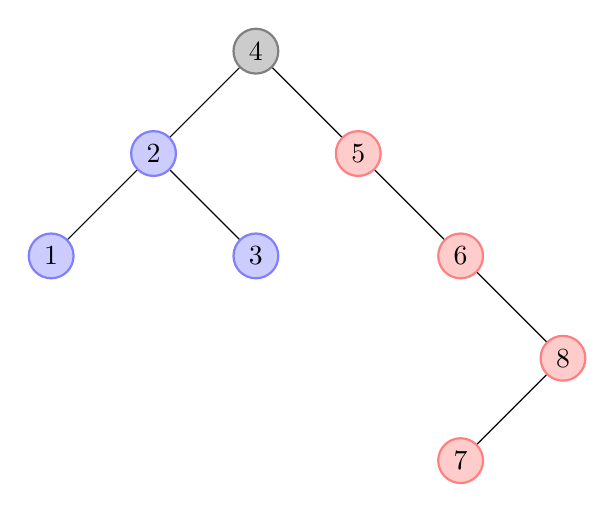
\begin{tikzpicture}
	[inner sep=1mm,
	normal/.style={circle,draw=blue!50,fill=blue!20,thick},
	visit/.style={circle,draw=red!50,fill=red!20,thick},
	roots/.style={circle,draw=black!50,fill=black!20,thick}]
	\node (4) at (0, 0) [roots] {4};
	\node (2) at (-1.3, -1.3) [normal] {2};
	\node (5) at (1.3, -1.3) [visit] {5};
	\node (6) at (2.6, -2.6) [visit] {6};
	\node (8) at (3.9, -3.9) [visit] {8};
	\node (7) at (2.6, -5.2) [visit] {7};
	\node (1) at (-2.6, -2.6) [normal] {1};
	\node (3) at (0, -2.6) [normal] {3};
	\draw [-] (4) to (2);
	\draw [-] (4) to (5);
	\draw [-] (2) to (1);
	\draw [-] (2) to (3);
	\draw [-] (5) to (6);
	\draw [-] (6) to (8);
	\draw [-] (8) to (7);
\end{tikzpicture}
\caption{The example figure}
\end{figure}
